% !TEX encoding = UTF-8 Unicode
% !TEX program = latexmk -xelatex
% !TEX root = ./main.tex
% !BIB program = biber

%----------------------------------------------------------------------------------------
% PACKAGES AND OTHER DOCUMENT CONFIGURATIONS
%----------------------------------------------------------------------------------------

\documentclass[
  UTF8, % Encoding
  12pt, % Default font size, values between 10pt-12pt are allowed
  % letterpaper, % Uncomment for US letter paper size
  % Chinese, % Uncomment for Chisese
]{assignment}

%----------------------------------------------------------------------------------------
% ASSIGNMENT INFORMATION
%----------------------------------------------------------------------------------------

\title{Homework \#1} % Assignment title

\author{Xuehai Pan} % Student name
\studentid{123456} % Student id

\date{Nov 11th, 2019} % Due date

\institute{School of Electronics Engineering and Computer Science \\ Peking University} % Institute or school name

\class{Special Relativity} % Course or class name

\lecturer{Dr. Albert Einstein} % Lecturer or teacher in charge of the assignment

%----------------------------------------------------------------------------------------

\begin{document}

\maketitle % Output the assignment title, created automatically using the information in the custom commands above

%----------------------------------------------------------------------------------------
% ASSIGNMENT CONTENT
%----------------------------------------------------------------------------------------

\section*{Question 1}

\begin{problem}
What is the airspeed velocity of an unladen swallow?
\end{problem}

\begin{figure}[H]
  \centering
  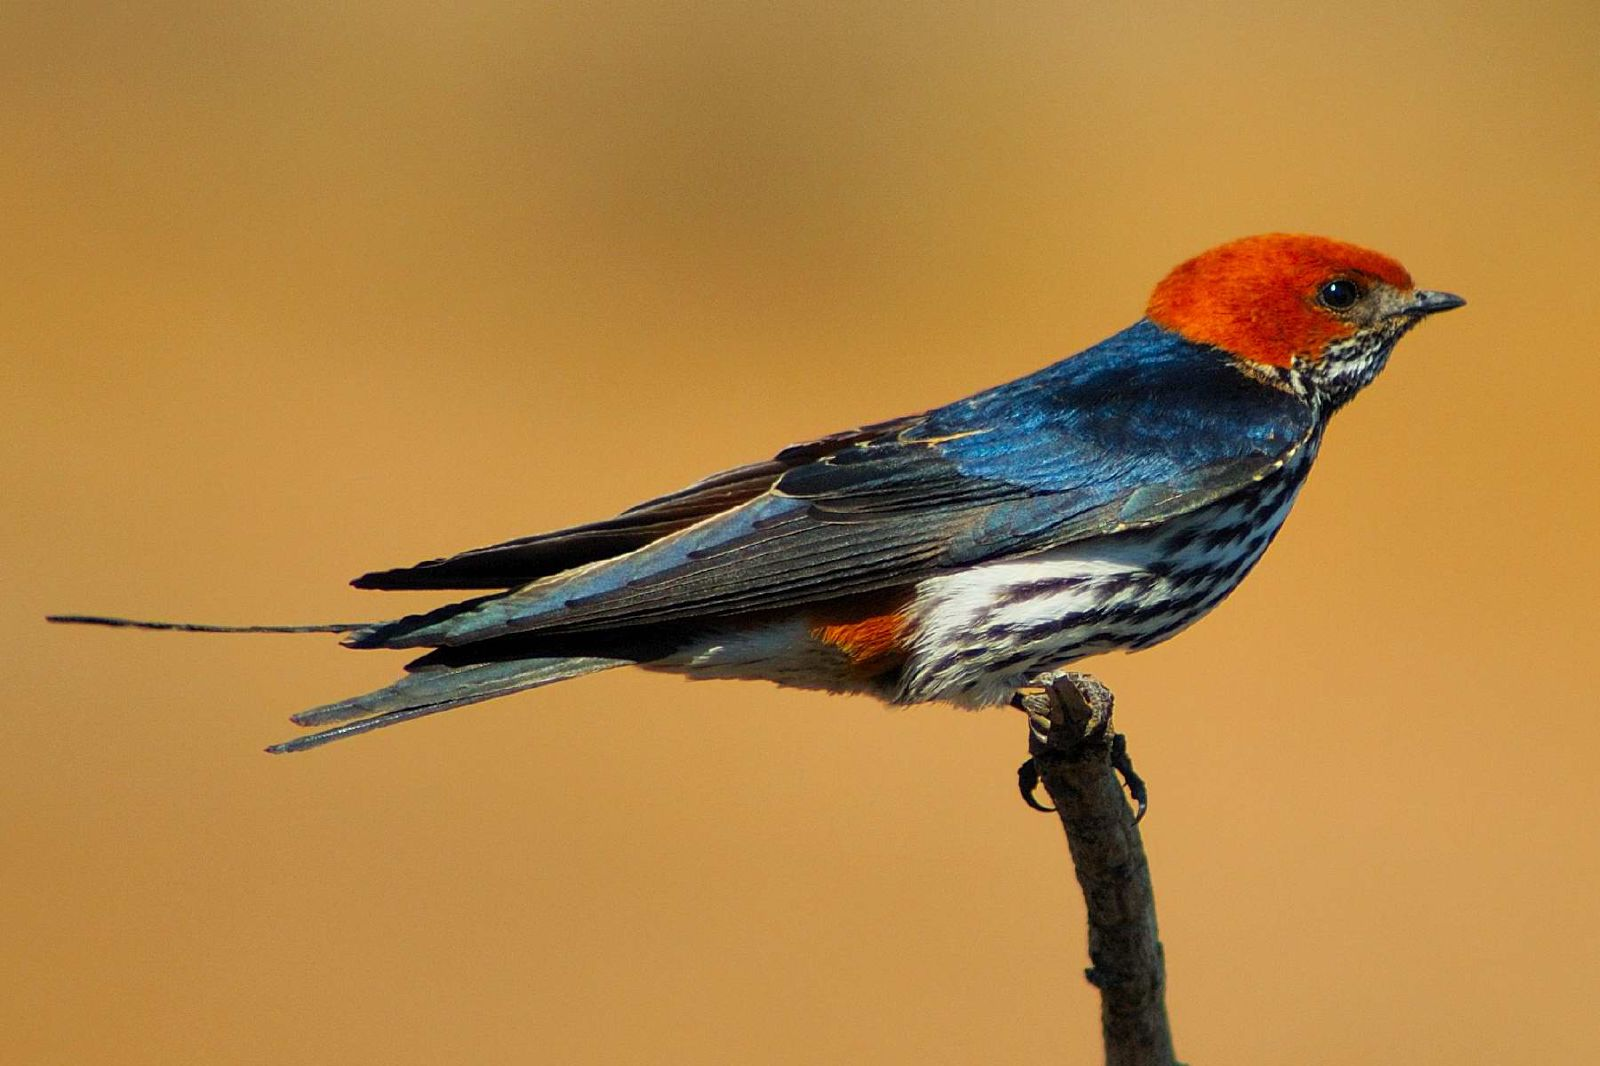
\includegraphics[width=0.5\columnwidth]{swallow.jpg} % Example image
  \caption{Swallow}
  \label{fig:swallow}
\end{figure}

\begin{figure}[H]
  \centering
  \begin{subfigure}[b]{0.4\textwidth}
    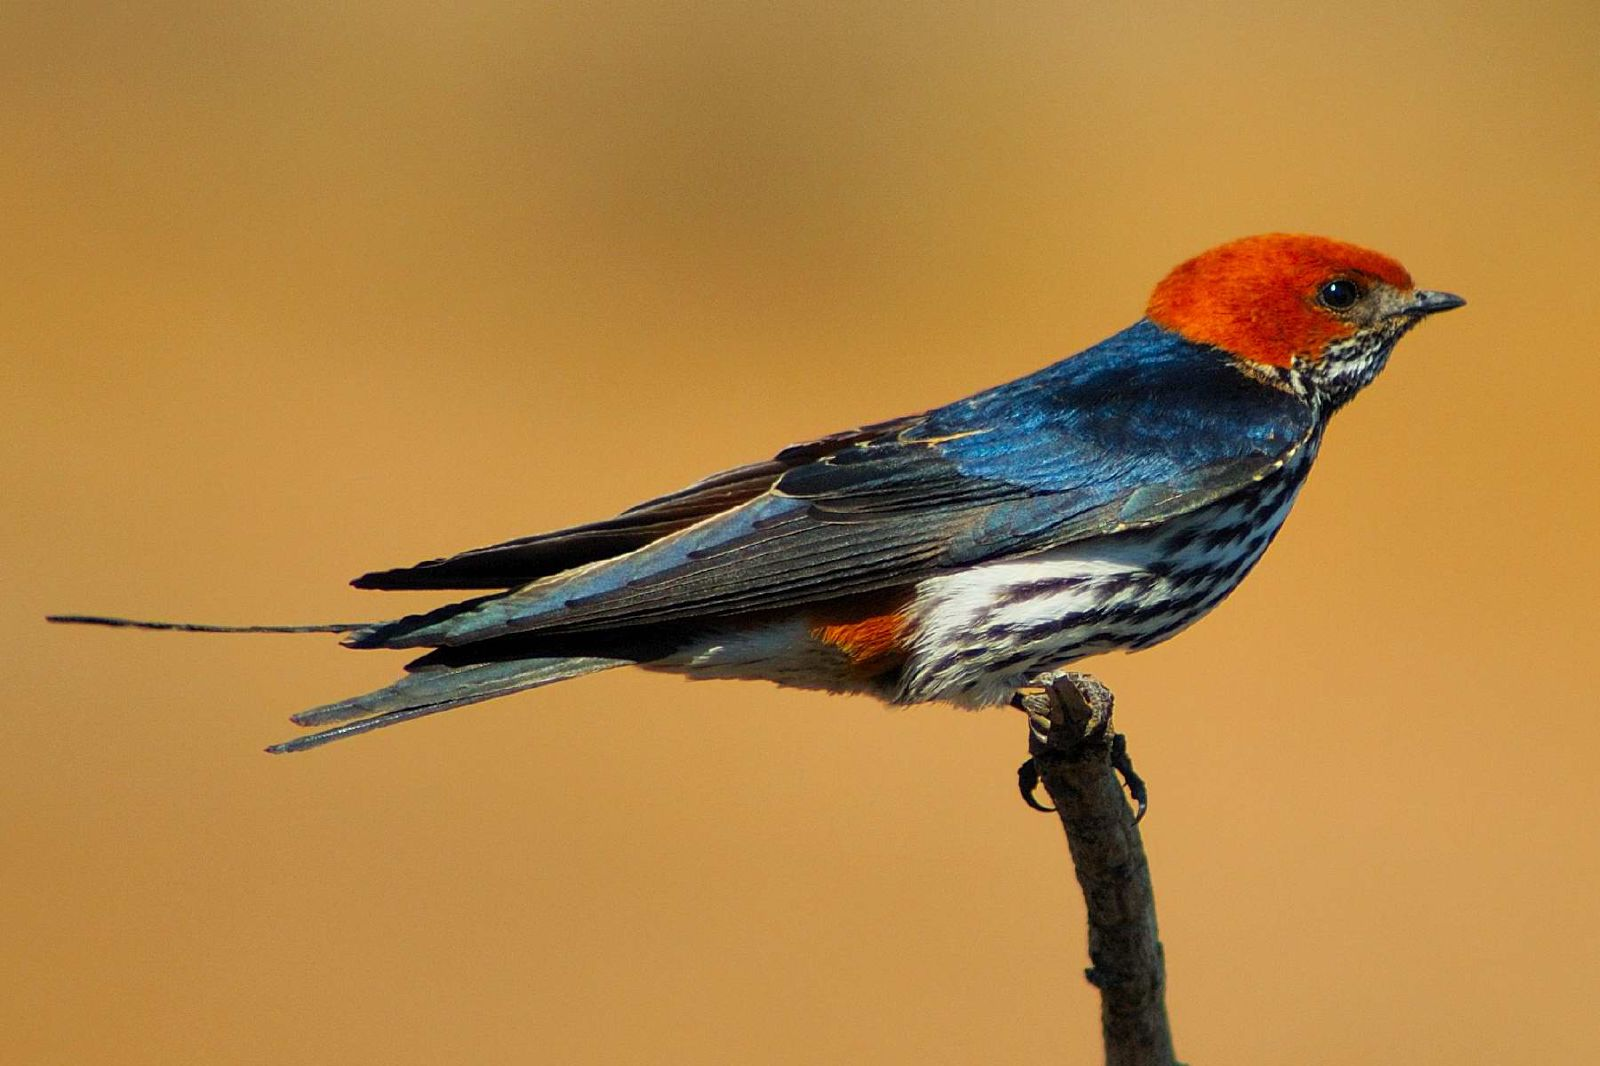
\includegraphics[width=\textwidth]{swallow.jpg}
    \caption{Swallow 1}
    \label{fig:swallow_1}
  \end{subfigure} \quad
  \begin{subfigure}[b]{0.4\textwidth}
    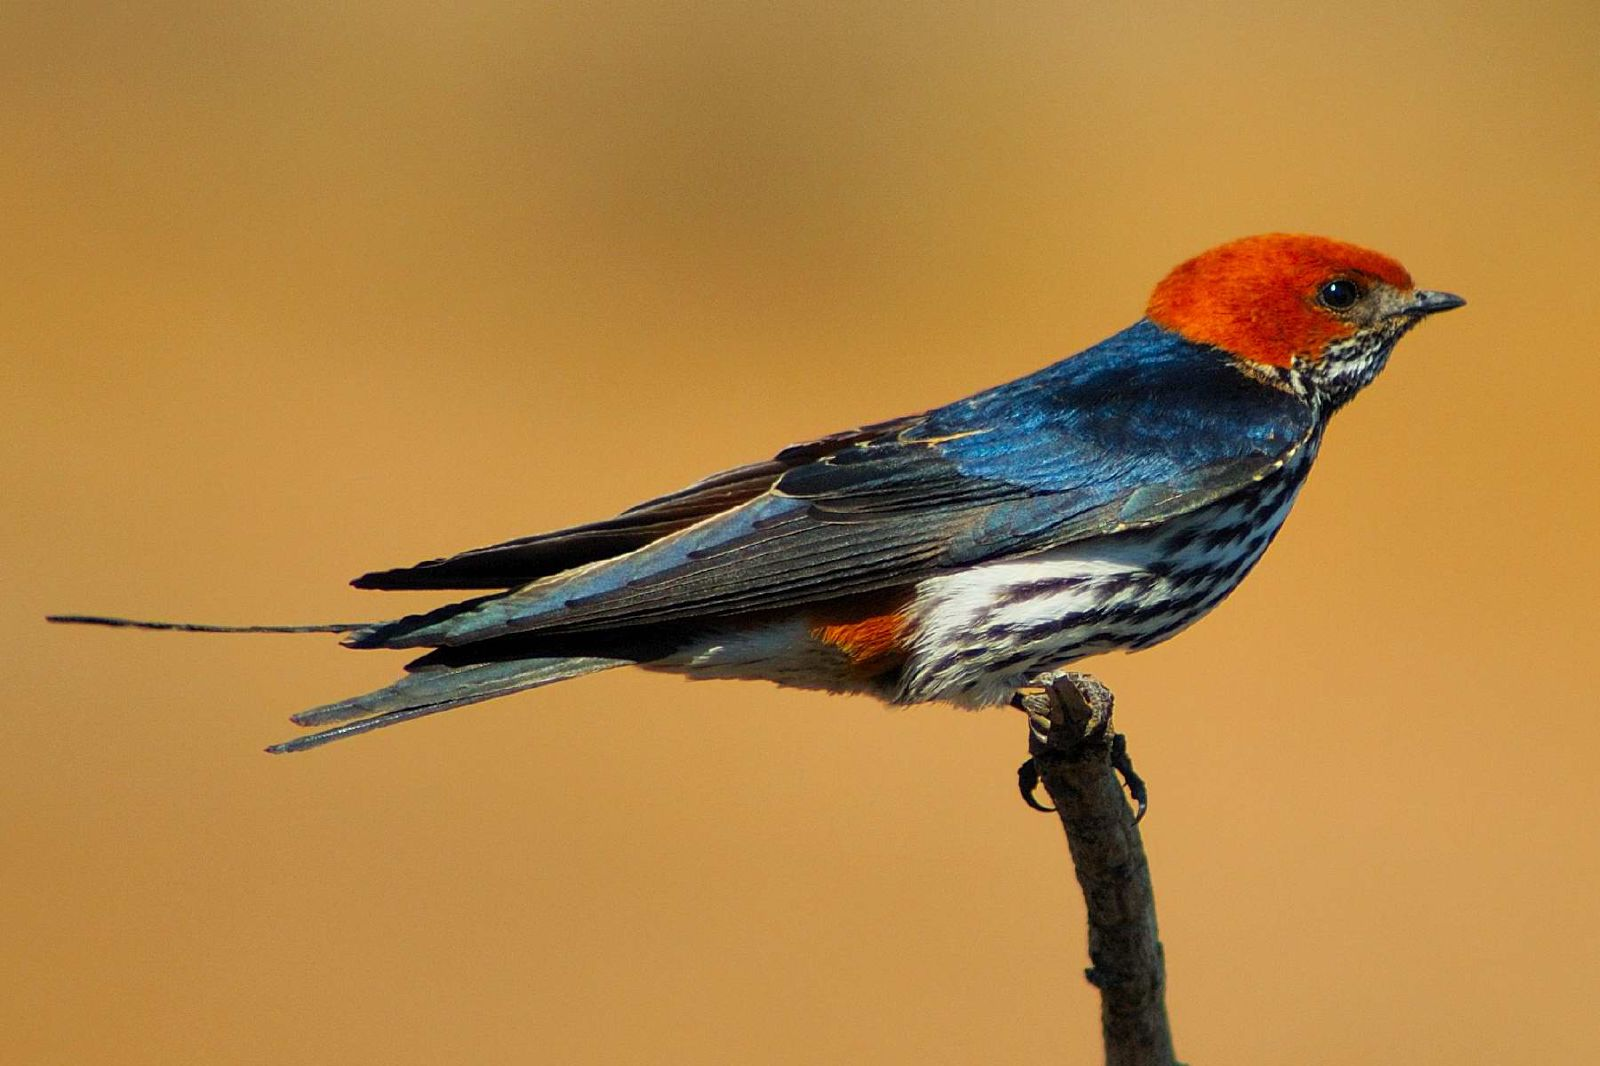
\includegraphics[width=\textwidth]{swallow.jpg}
    \caption{Swallow 2}
    \label{fig:swallow_2}
  \end{subfigure}
  \caption{Swallow}
  \label{fig:swallow_all}
\end{figure}

%------------------------------------------------

\subsection*{Solution}

While this question leaves out the crucial element of the geographic origin of the swallow, according to Jonathan Corum, an unladen European swallow maintains a cruising airspeed velocity of \textbf{11 metres per second}, or \textbf{24 miles an hour}. The velocity of the corresponding African swallows requires further research as kinematic data is severely lacking for these species.

%----------------------------------------------------------------------------------------

\section*{Question 2}

\begin{problem}
How much wood would a woodchuck chuck if a woodchuck could chuck wood?

\medskip

\begin{enumerate}[label=(\emph{\alph*}), ref=\alph*] % Sub-questions styled as italic letters
  \item Suppose "chuck" implies throwing.
  \item Suppose "chuck" implies vomiting.
\end{enumerate}
\end{problem}

%------------------------------------------------

\subsection*{Solution}

\begin{enumerate}[label=(\emph{\alph*}), ref=\alph*] % Sub-questions styled as italic letters
  \item According to the Associated Press (1988), a New York Fish and Wildlife technician named Richard Thomas calculated the volume of dirt in a typical 25--30 foot (7.6--9.1 m) long woodchuck burrow and had determined that if the woodchuck had moved an equivalent volume of wood, it could move ``about \textbf{700 pounds (320 kg)} on a good day, with the wind at his back".

  \item A woodchuck can ingest 361.92 cm\textsuperscript{3} (22.09 cu in) of wood per day. Assuming immediate expulsion on ingestion with a 5\% retainment rate, a woodchuck could chuck \textbf{343.82 cm\textsuperscript{3}} of wood per day.
\end{enumerate}

%----------------------------------------------------------------------------------------

\section*{Question 3}

\begin{problem}
Identify the author of Equation \eqref{eq:bayes} below and briefly describe it in Latin.

\medskip

\begin{equation}\label{eq:bayes}
  P \qty( A \middle| B ) = \frac{ P \qty( B \middle| A ) \, P (A)}{P (B)}
\end{equation}

\smallskip
\end{problem}

%------------------------------------------------

\subsection*{Solution}

Lorem ipsum dolor sit amet, consectetur adipiscing elit. Praesent porttitor arcu luctus, imperdiet urna iaculis, mattis eros. Pellentesque iaculis odio vel nisl ullamcorper, nec faucibus ipsum molestie. Sed dictum nisl non aliquet porttitor. Etiam vulputate arcu dignissim, finibus sem et, viverra nisl. Aenean luctus congue massa, ut laoreet metus ornare in. Nunc fermentum nisi imperdiet lectus tincidunt vestibulum at ac elit. Nulla mattis nisl eu malesuada suscipit.

%----------------------------------------------------------------------------------------

\section*{Question 4 (bonus marks)}

\begin{problem}
The table below shows the nutritional consistencies of two sausage types. Explain their relative differences given what you know about daily adult nutritional recommendations.

\bigskip

\begin{table}[H]
  \centering
  \caption{Daily Adult Nutritional Recommendations}
  \label{tab:nutritional_recommendations}
  \begin{tabular}{|l|l|l|}
    \toprule
    \textit{Per 50g} & Pork  & Soy   \\
    \midrule
    Energy           & 760kJ & 538kJ \\
    Protein          & 7.0g  & 9.3g  \\
    Carbohydrate     & 0.0g  & 4.9g  \\
    Fat              & 16.8g & 9.1g  \\
    Sodium           & 0.4g  & 0.4g  \\
    Fibre            & 0.0g  & 1.4g  \\
    \bottomrule
  \end{tabular}
\end{table}

\medskip
\end{problem}

%------------------------------------------------

\subsection*{Solution}

Lorem ipsum dolor sit amet, consectetur adipiscing elit. Praesent porttitor arcu luctus, imperdiet urna iaculis, mattis eros. Pellentesque iaculis odio vel nisl ullamcorper, nec faucibus ipsum molestie. Sed dictum nisl non aliquet porttitor. Etiam vulputate arcu dignissim, finibus sem et, viverra nisl. Aenean luctus congue massa, ut laoreet metus ornare in. Nunc fermentum nisi imperdiet lectus tincidunt vestibulum at ac elit. Nulla mattis nisl eu malesuada suscipit.

%----------------------------------------------------------------------------------------

\section*{Question 5 (bonus marks)}

\begin{problem}
\begin{code}
  \caption{Luftballons Perl Script} % Caption above the listing
  \inputminted[
    label=Luftballons Perl Script, % Add a label to the top, the bottom or both of the frames around the code
  ]{perl}{luftballons.pl}
  \label{lst:luftballons} % Label for referencing this listing
\end{code}

\begin{enumerate}[label=(\arabic*), ref=\arabic*]
  \item How many luftballons will be output by the Listing \ref{lst:luftballons} above?
  \item Identify the regular expression in Listing \ref{lst:luftballons} and explain how it relates to the anti-war sentiments found in the rest of the script.
\end{enumerate}

\end{problem}

%------------------------------------------------

\subsection*{Solution}

\begin{enumerate}[label=(\arabic*), ref=\arabic*]
  \item 99 luftballons.
  \item Lorem ipsum dolor sit amet, consectetur adipiscing elit. Praesent porttitor arcu luctus, imperdiet urna iaculis, mattis eros. Pellentesque iaculis odio vel nisl ullamcorper, nec faucibus ipsum molestie. Sed dictum nisl non aliquet porttitor. Etiam vulputate arcu dignissim, finibus sem et, viverra nisl. Aenean luctus congue massa, ut laoreet metus ornare in. Nunc fermentum nisi imperdiet lectus tincidunt vestibulum at ac elit. Nulla mattis nisl eu malesuada suscipit.
\end{enumerate}

%----------------------------------------------------------------------------------------

\end{document}
